% Created by Baoyun Ge on 5/2/20.
% Copyright © 2020 Baoyun Ge. All rights reserved.
\documentclass[letterpaper, 10pt]{article}

\usepackage[noadjust]{cite}
\usepackage{color}
\usepackage{amsmath}
\usepackage{graphicx}
\usepackage{caption}
\usepackage{subcaption}
\usepackage{cuted}
% \usepackage{hyperref}
\usepackage[nameinlink]{cleveref}
\usepackage[flushleft, para]{threeparttable}
\usepackage{multirow}
\usepackage{booktabs}
\usepackage{nth}
\usepackage{afterpage}
\usepackage{contour}

\usepackage{tikz}
\usepackage{circuitikz}
\usepackage{pgfplots}
\pgfplotsset{compat = 1.12}

\usetikzlibrary{datavisualization.formats.functions}
\usetikzlibrary{plotmarks}
\usetikzlibrary{math}
\usetikzlibrary{calc}
\usetikzlibrary{spy}
\usetikzlibrary{positioning}
\usetikzlibrary{intersections}
\usetikzlibrary{decorations.text}
\usetikzlibrary{external}
\usetikzlibrary{patterns}
\usetikzlibrary{arrows.meta}
\usetikzlibrary{arrows}
\usetikzlibrary{matrix}

\tikzexternalize

\pgfplotsset{
    legend image with text/.style={
        legend image code/.code={%
            \node[anchor=center] at (0.3cm,0cm) {#1};
        }
    },
}

\mathchardef\myhyphen="2D

\begin{document}

\ifpdf
\DeclareGraphicsExtensions{.pdf, .jpg, .tif}
\else
\DeclareGraphicsExtensions{.eps, .jpg}
\fi

\tikzsetexternalprefix{images/tikz/}

\begin{figure}
  \centering
  \tikzsetnextfilename{tikz-legend-matrix}
  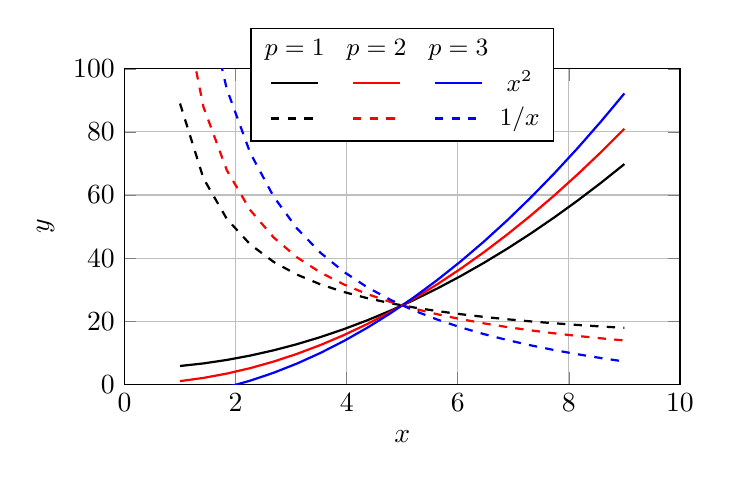
\begin{tikzpicture}
    \begin{axis}
    [
      width = 3.4in,
      height = 2.2in,
      xlabel = {$x$},
      ylabel = {$y$},
      xtick = {0, 2, 4, 6, 8, 10},
      ytick = {0, 20, 40, 60, 80, 100},
      xmin = 0, xmax = 10,
      ymin = 0, ymax = 100,
      grid = major,
      legend style = {at = {(axis cs: 5, 95)}, anchor = center, font = \small, legend columns = 3},
    ]
    
    % first row of the legend matrix
    \addlegendimage{legend image with text={$p=1$}}
    \addlegendentry{}
    
    \addlegendimage{legend image with text={$p=2$}}
    \addlegendentry{}    
    
    \addlegendimage{legend image with text={$p=3$}}
    \addlegendentry{}
    
    % second row
    \addplot [thick, black, domain = 1:9, samples = 20] {0.8 * x^2 + 5.0};
    \addlegendentry{}
    \addplot [thick, red, domain = 1:9, samples = 20] {1.0 * x^2 + 0.0};
    \addlegendentry{}
    \addplot [thick, blue, domain = 1:9, samples = 20] {1.2 * x^2 - 5.0};
    \addlegendentry{$x^{2}$}
    
    % third row
    \addplot [thick, black, dashed, domain = 1:9, samples = 20] {80 / x + 9.0}; 
    \addlegendentry{}   
    \addplot [thick, red, dashed, domain = 1:9, samples = 20] {125 / x};
    \addlegendentry{}
    \addplot [thick, blue, dashed, domain = 1:9, samples = 20] {200 / x - 15.0};
    \addlegendentry{$1/x$}
    \end{axis}
  \end{tikzpicture}
\end{figure}

\end{document}


%%% Local Variables:
%%% mode: latex
%%% TeX-master: t
%%% TeX-command-extra-options: "-shell-escape"
%%% End:
